% Created 2017-03-01 Wed 20:38
\documentclass[10pt]{article}
\usepackage[utf8]{inputenc}
\usepackage[T1]{fontenc}
\usepackage{fixltx2e}
\usepackage{graphicx}
\usepackage{longtable}
\usepackage{float}
\usepackage{wrapfig}
\usepackage{rotating}
\usepackage[normalem]{ulem}
\usepackage{amsmath}
\usepackage{textcomp}
\usepackage{marvosym}
\usepackage{wasysym}
\usepackage{amssymb}
\tolerance=1000
\usepackage{natbib}
\usepackage[linktocpage,pdfstartview=FitH,colorlinks,
linkcolor=blue,anchorcolor=blue,
citecolor=blue,filecolor=blue,menucolor=blue,urlcolor=blue]{hyperref}
\usepackage[margin=2cm]{geometry}
\pagenumbering{gobble}
\usepackage{wrapfig}
\usepackage{multicol}
\setlength\columnsep{20pt}
\author{Alejandro Rodríguez Salamanca: r0650814@student.kuleuven.be}
\date{}


\title{Artificial Neural Networks: Session 3}
\begin{document}

\maketitle

\begin{multicols}{2}
  \section*{Handwritten Digits PCA and reconstruction}
  In this exercise we are asked to perform PCA on handwritten images
  of the digit 3 taken from the US Postal Service database.
  First of all, the mean is displayed. This plot shows the mean of each column
  of the input data.

  % PLOT OF THE MEAN
  \begin{center}
	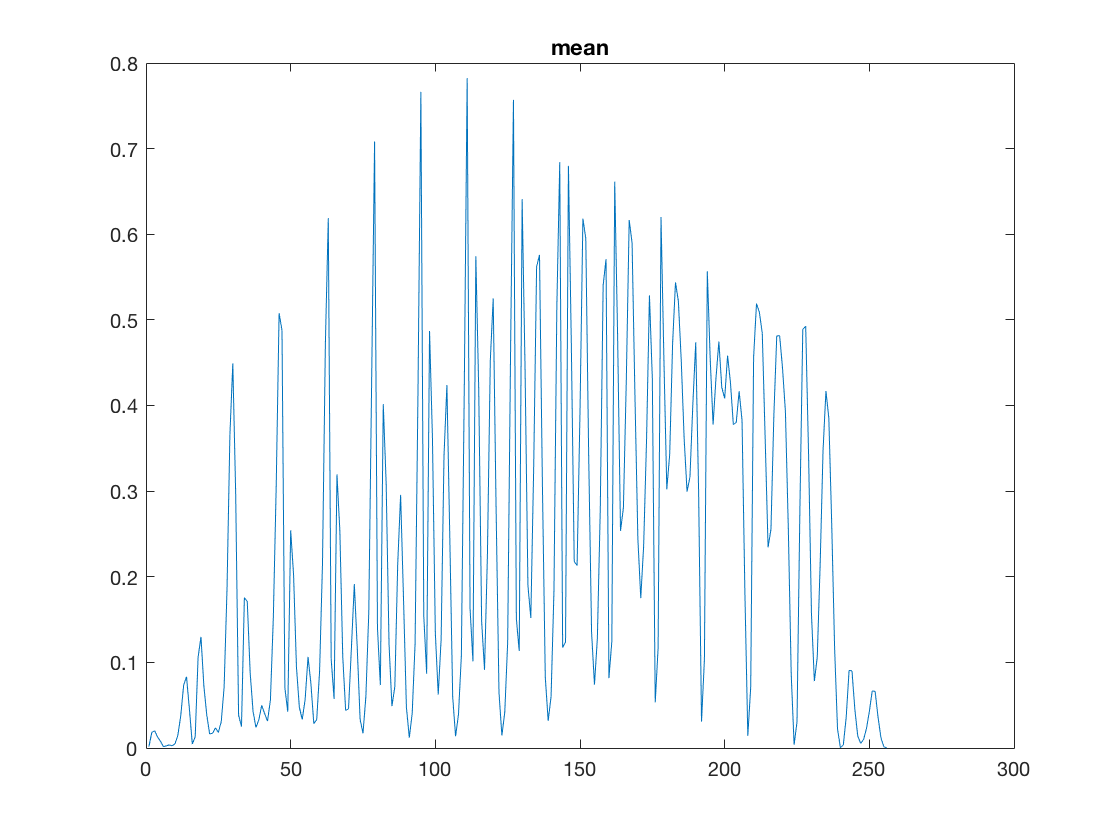
\includegraphics[width=0.8\linewidth]{img/mean}
  \end{center}

  It can be seen that the mean varies across the columns without showing any
  recognizable pattern.

  This second plot shows the eigenvalues of the covariance matrix of the
  input data.

  % PLOT OF COVARIANCE
  \begin{center}
	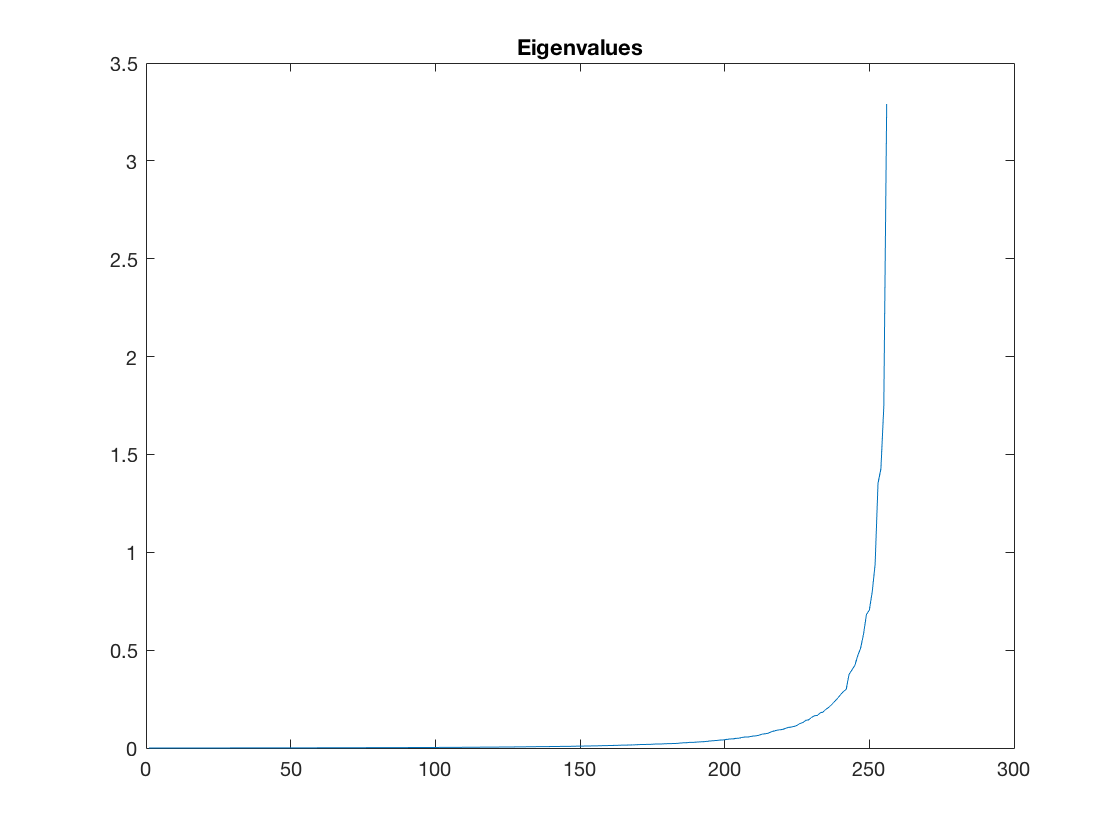
\includegraphics[width=0.8\linewidth]{img/eig}
  \end{center}

  Then, the Principal Component Analysis is computed. The objective is to reduce the
  dimensionality of our data. For this, it is decomposed into its principal components,
  and then, the number of components to use is deceided. This plot represents the
  significance of each component in the original data. As we can see,
  few of the components capture most of the variance of the data, which means that it
  is possible to get rid of most of the dimensions, reducing cosinderably the complexity
  of our dataset.

  The following image shows the original digit 3 of the data set used, and below, we can see
  the reconstruction of this digit after projecting the original data set into one, two,
  three and four principal components.

  % ORIGINAL IMAGE
  \begin{center}
	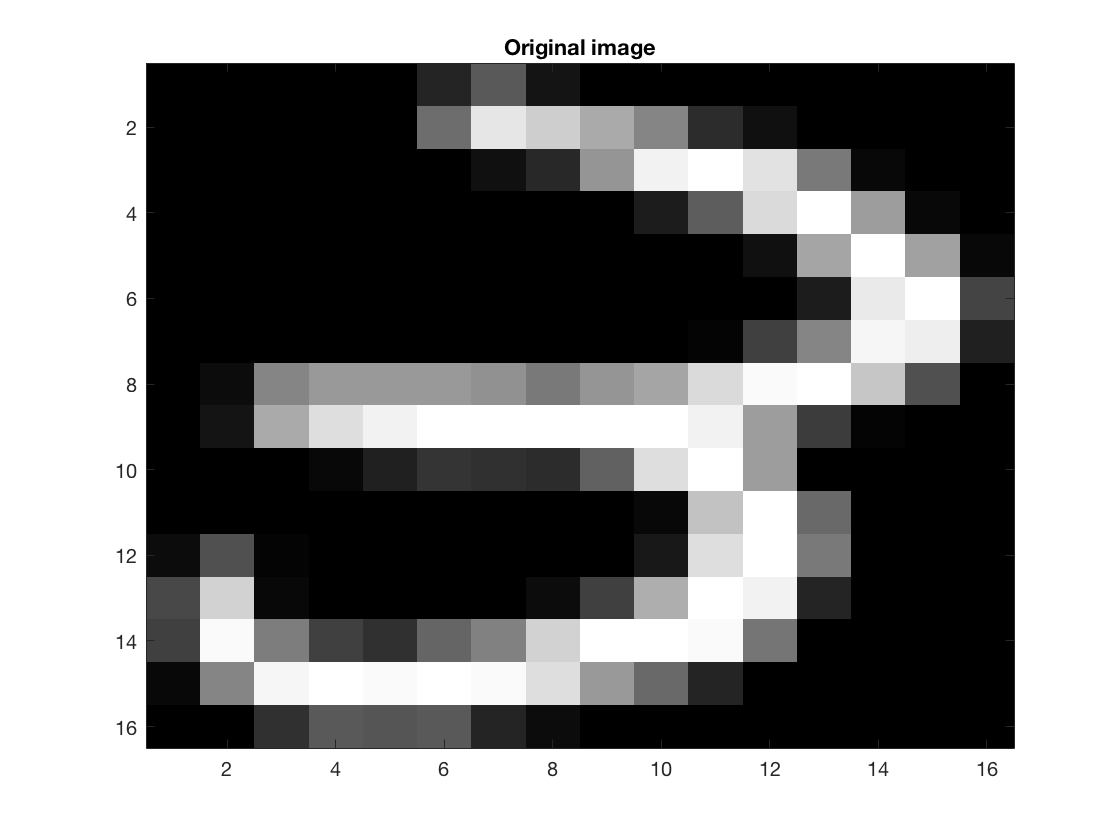
\includegraphics[width=0.5\linewidth]{img/threeorig}
  \end{center}

  % RECONSTRUCTED IMAGES
  \begin{center}
	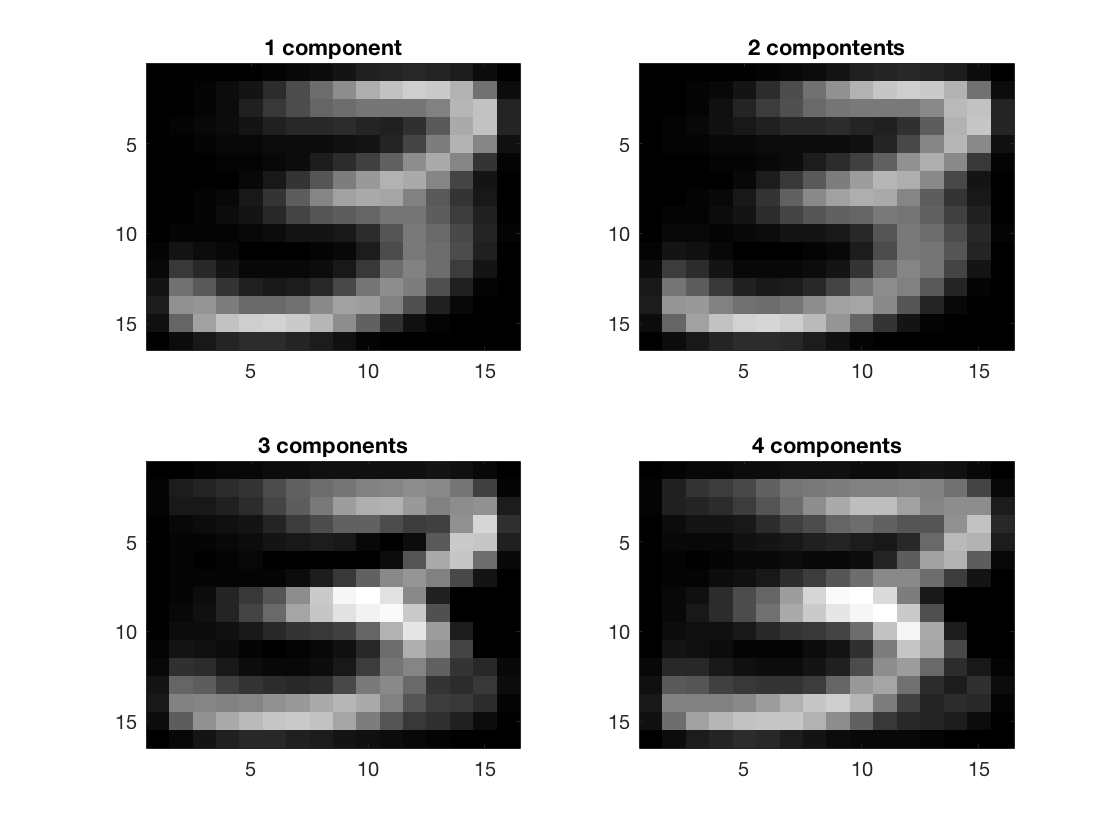
\includegraphics[width=0.8\linewidth]{img/threerec}
  \end{center}

  At first glance it is difficult to see how well the data has been reconstructed. Although
  it can be observed that the quality of the image increases with the number of components
  used, it is interesting to plot the error to see how it evolves.

  To achieve this, we have calculated the error as \texttt{sqrt(mean(mean((X-Xapprox)$^2$)))}.
  The inner \texttt{mean} is used to obtain the mean of each column of the matrix, and the
  outter \texttt{mean} to compute the mean of this new matrix, reducing it to a single value
  that we can plot, being \texttt{X} the original data set, and \texttt{Xapprox} the new
  approximated data set.

  The error have been computed iteratively using one more component on each iteration, starting
  at 1 and ending at 50 components.

  It is possible to see that the error function converges somewhere near \texttt{0.08},
  which means that using more than 50 components does not increase the quality of the
  reconstructed image, but only add more complexity to the data adding superfluous
  dimensions.

    % PLOT OF ERROR
  \begin{center}
	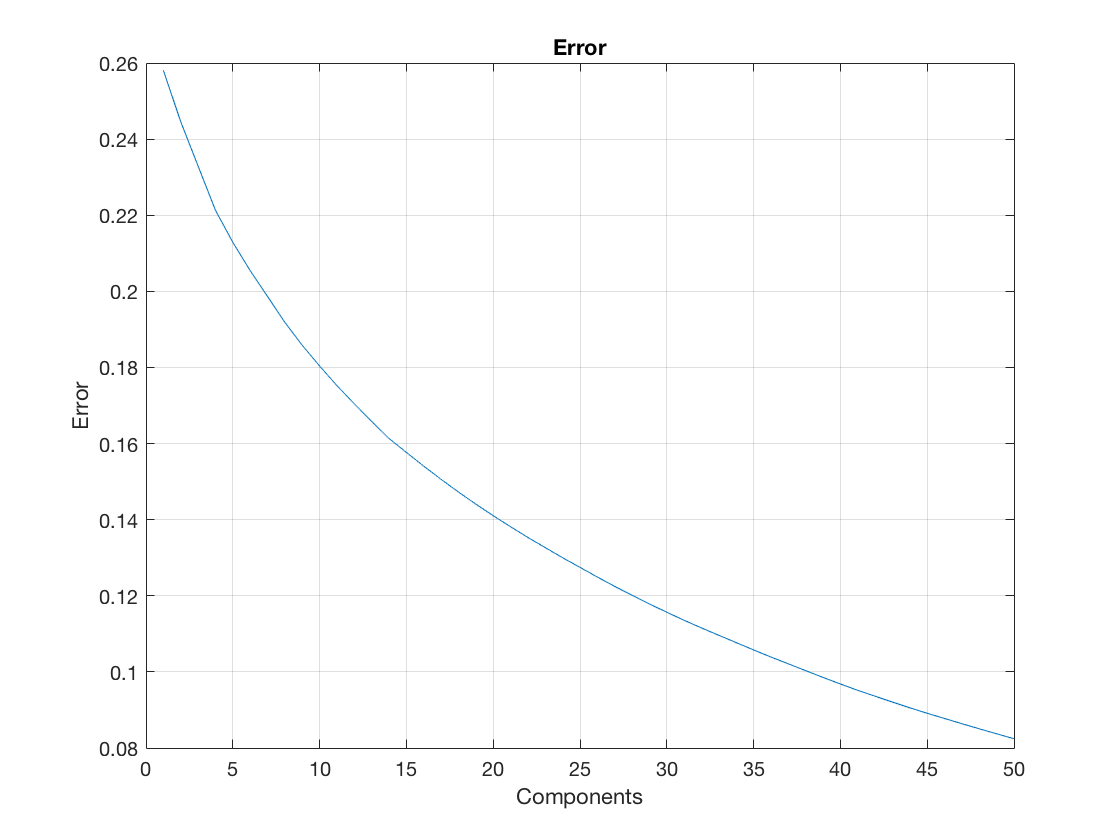
\includegraphics[width=0.8\linewidth]{img/error}
  \end{center}

  If we reconstruct with 256 principal components, this is, the whole matrix, the error
  should be zero, as we are using the entire matrix to reconstruct the original data, which
  means that there is no dimensionality reduction, but only a change of basis.

  In practice, this is not true, and we can see that the error is \texttt{0.0824}. This can be
  caused by the error carried by the operations in floating point.

  %TODO CUMSUM
  
  
  \section*{SOM applied to the cylinder and Iris datasets}
  A self ogranizing map is trained using unsupervised learning to produce
  a low-dimensional, discretized representation of the input space of the
  training samples. SOMs accomplish two things, they reduce dimensions and
  display similarities.
  \subsection*{Cylinders}
  In this example we generate data uniformely distributed within two concentric cylinders.
  The following images shows the neurons in three different topologies,
  \texttt{hextop, gridtop} and \texttt{randtop}.

  \begin{center}
    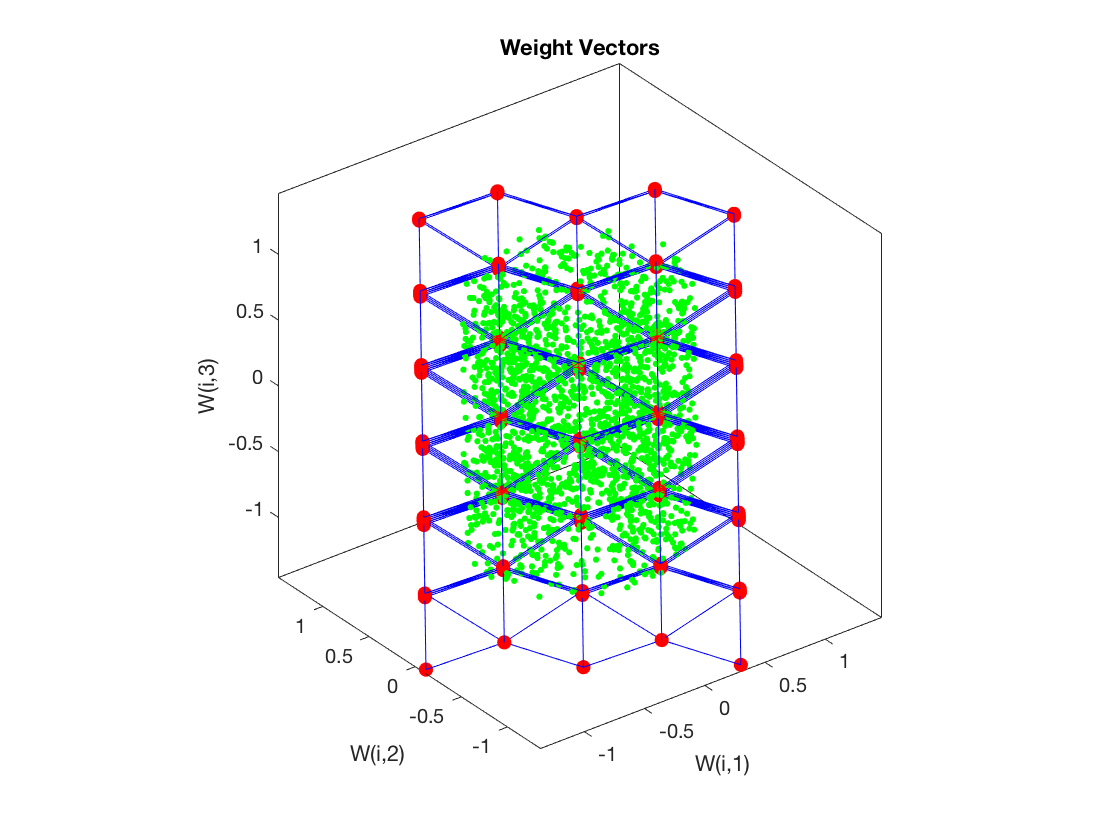
\includegraphics[width=0.49\linewidth]{img/somcylinderhexbefore}
    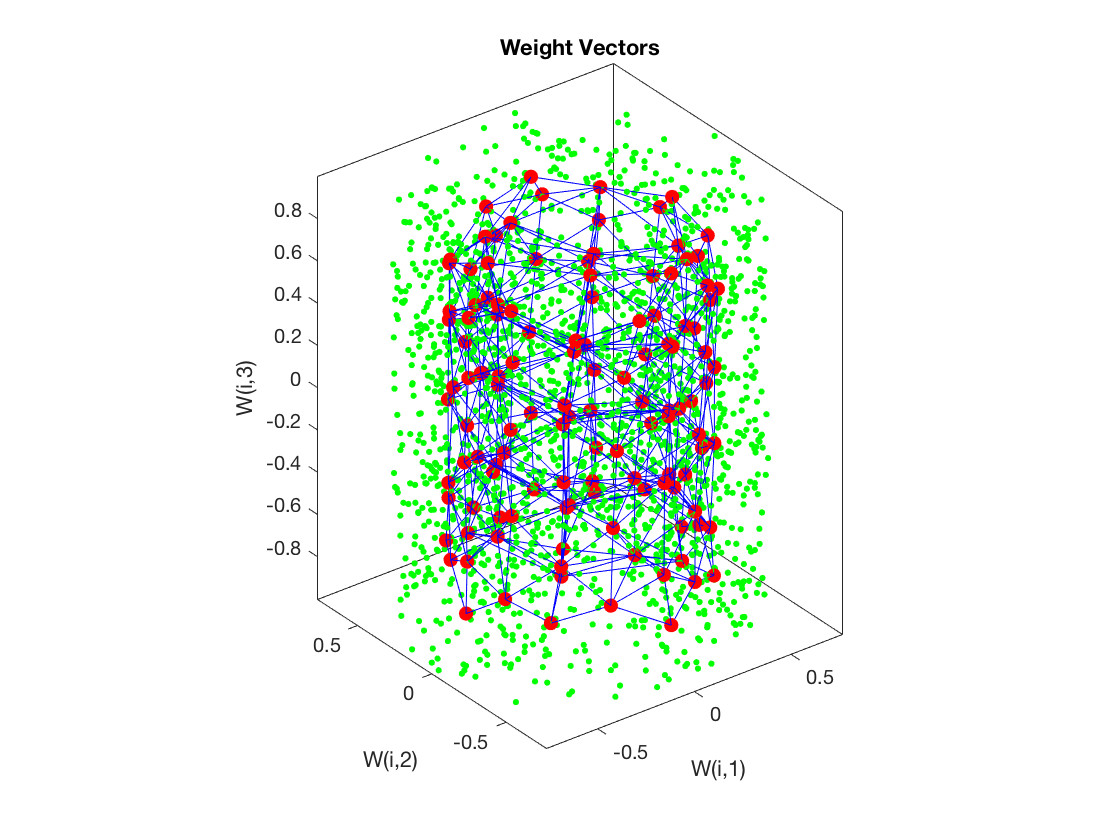
\includegraphics[width=0.49\linewidth]{img/somcylinderhexafter}
  \end{center}

  \begin{center}
    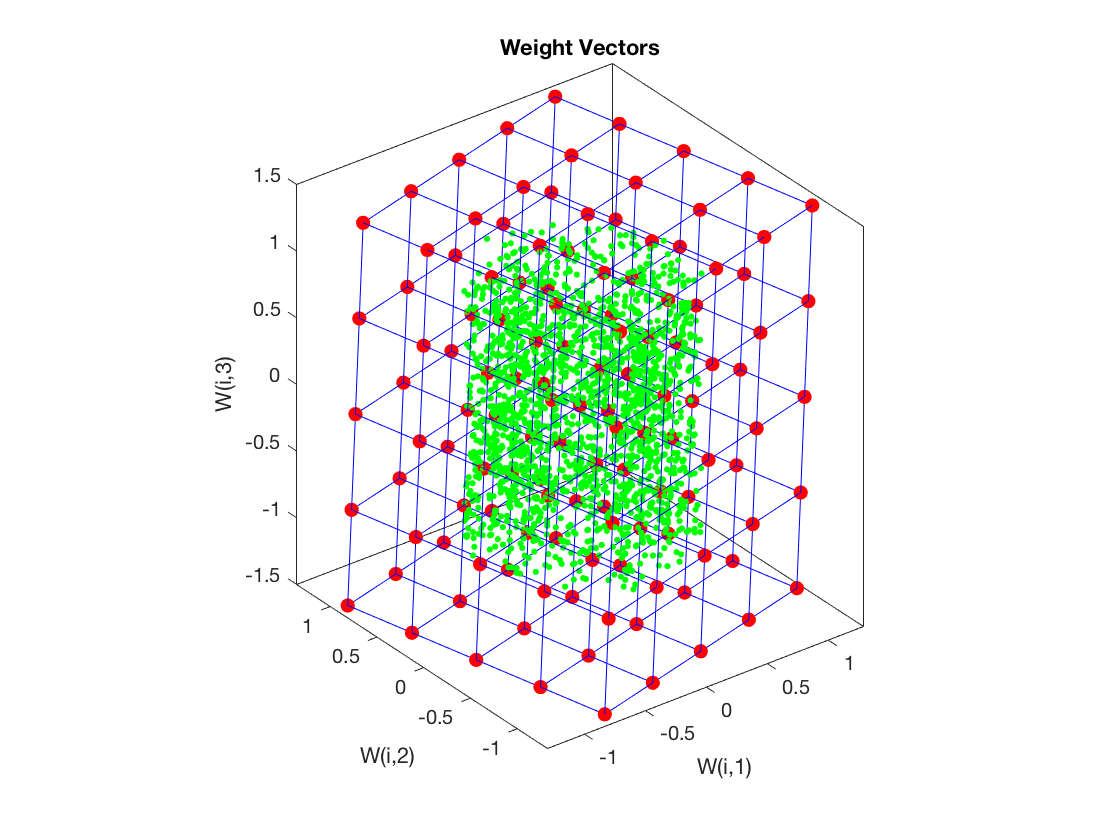
\includegraphics[width=0.49\linewidth]{img/somcylindertopbefore}
    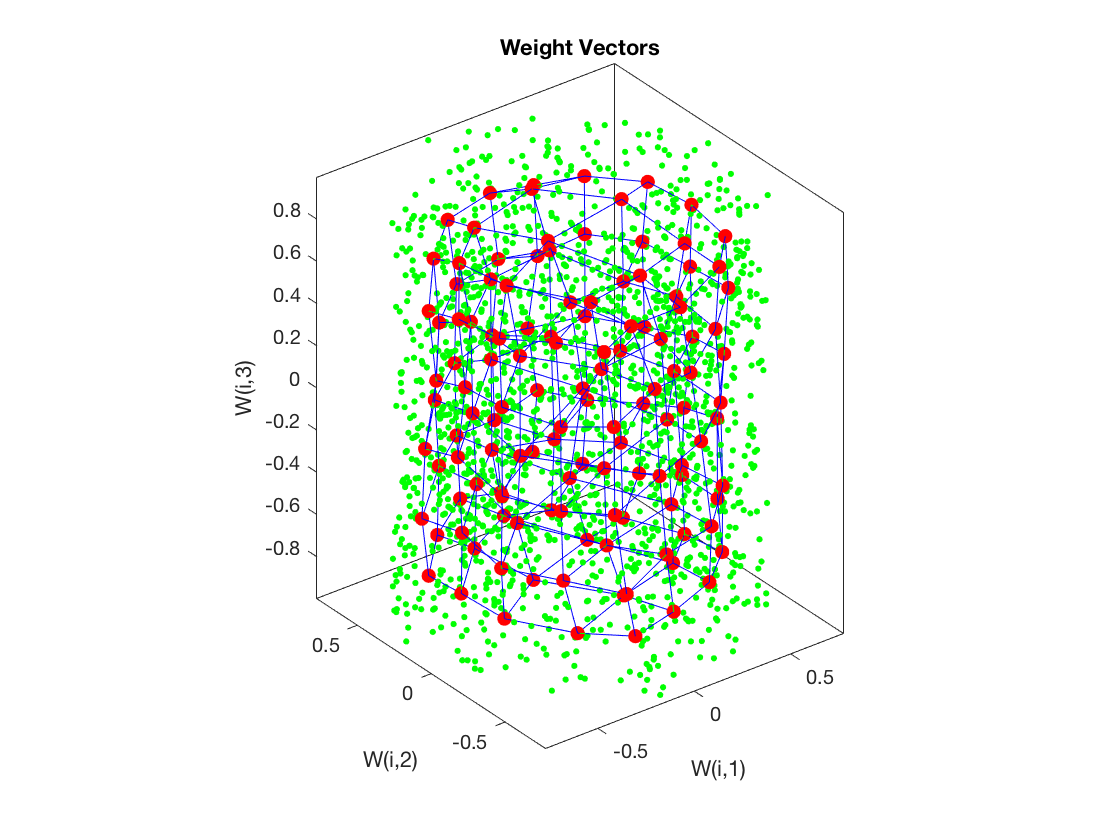
\includegraphics[width=0.49\linewidth]{img/somcylindertopafter}
  \end{center}

  \begin{center}
    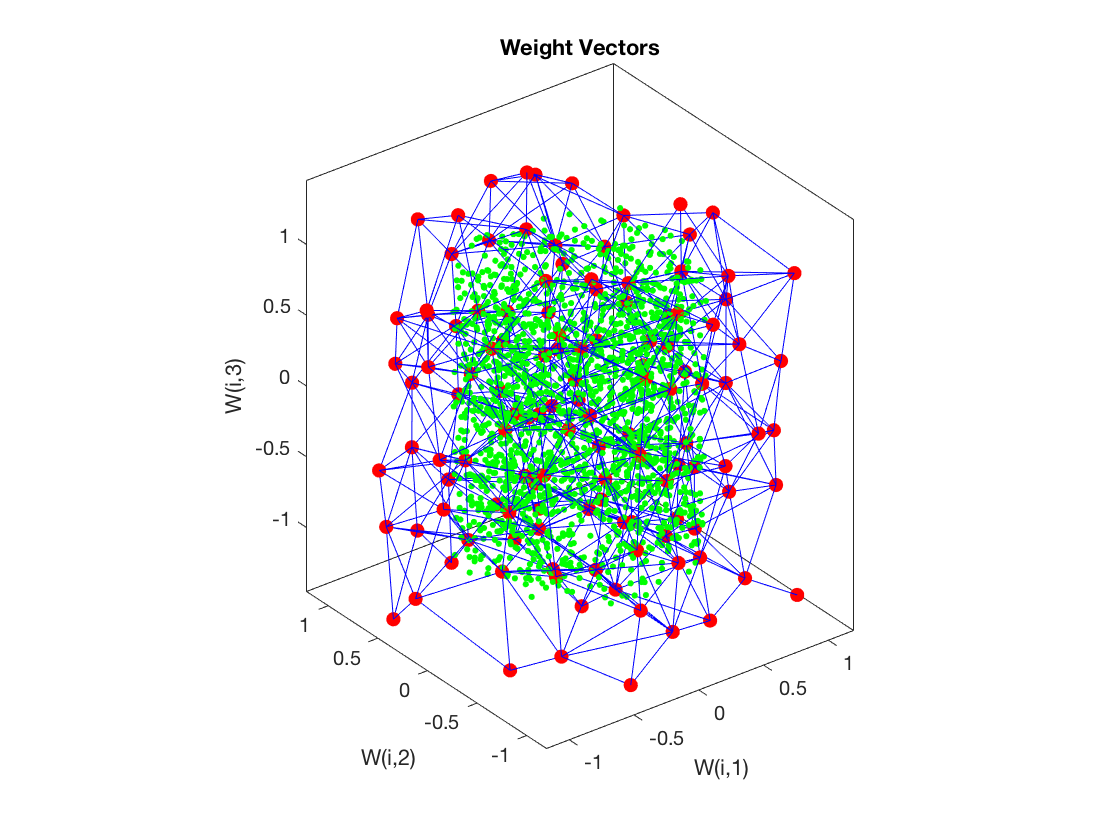
\includegraphics[width=0.49\linewidth]{img/somcylinderrandbefore}
    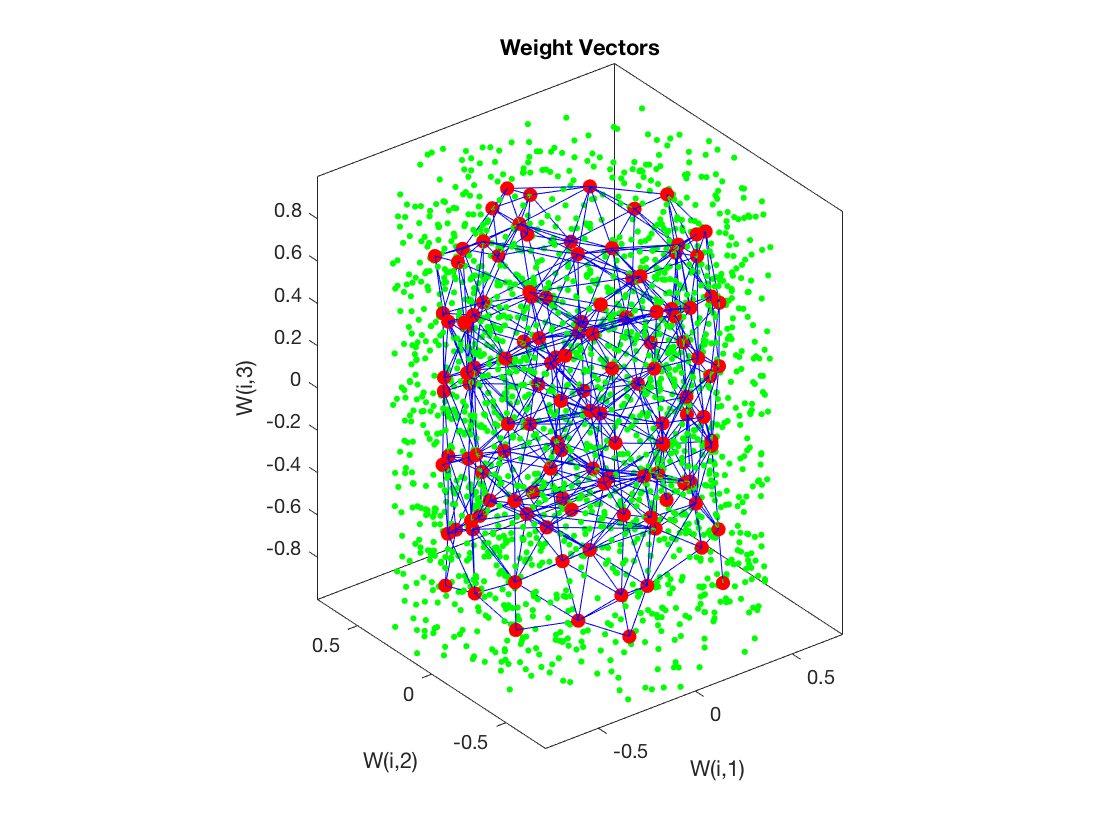
\includegraphics[width=0.49\linewidth]{img/somcylinderrandafter}
  \end{center}

  It is possible to see the difference in the initial disposition of the
  neurons depending on the selected topology, and how the neurons are arranged
  after training.

  It is also interesing to see the influence of the distance function used and how it affects
  to the final result. Here, \texttt{boxdist, dist} and \texttt{mandist} have been used.

  \begin{center}
    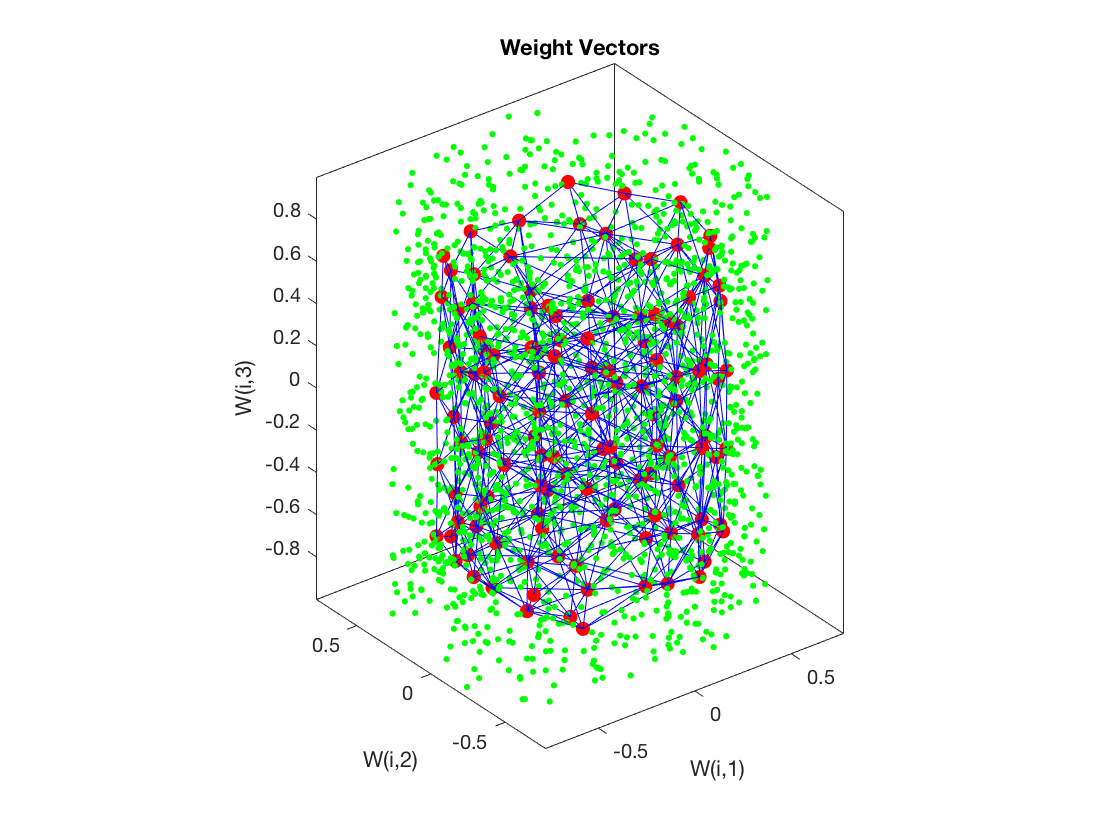
\includegraphics[width=0.32\linewidth]{img/somcylinderhexafterbox}
    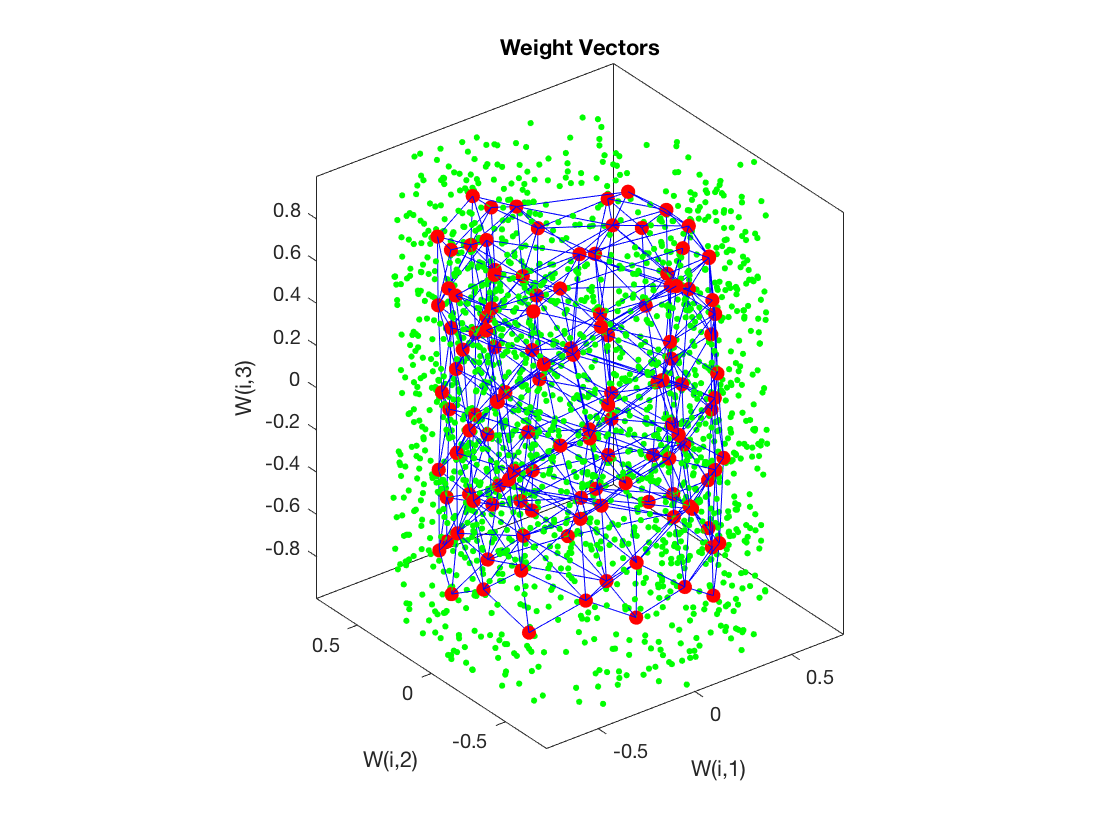
\includegraphics[width=0.32\linewidth]{img/somcylinderhexafterdist}
    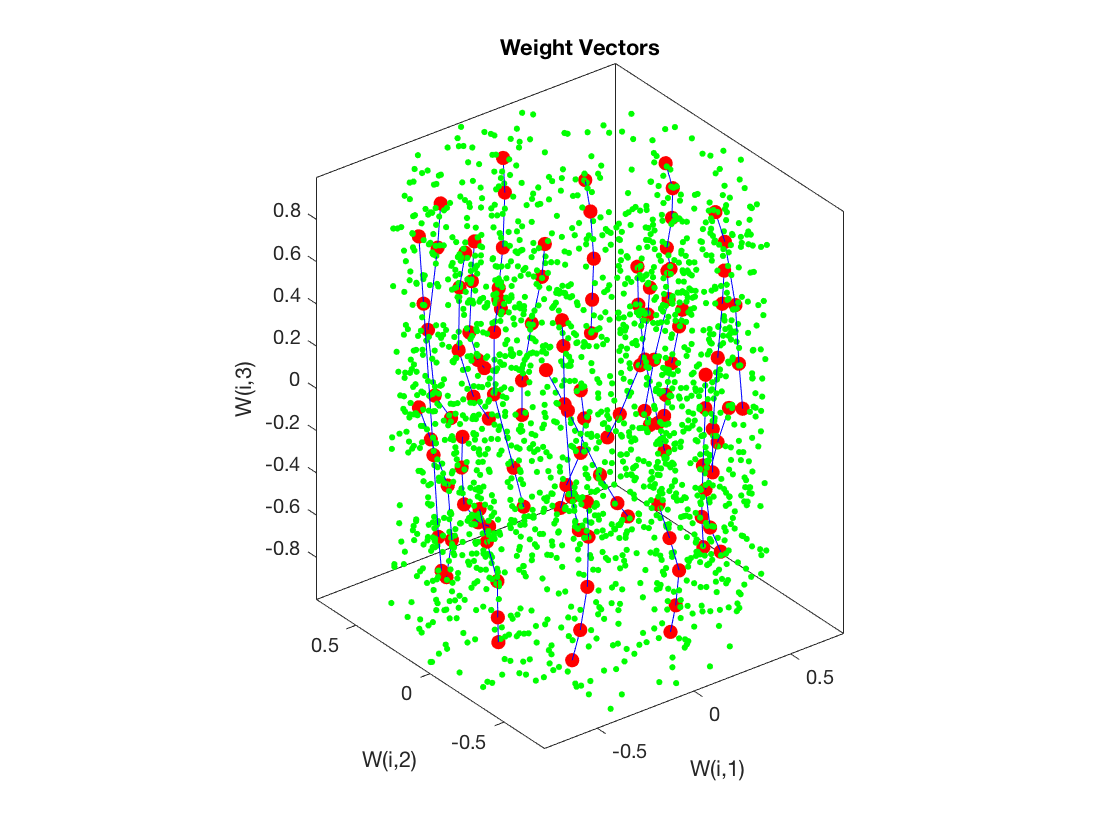
\includegraphics[width=0.32\linewidth]{img/somcylinderhexafterman}
  \end{center}
  
  \subsection*{Iris}
  The data set consists of samples from each of three species of Iris
  (Iris setosa, Iris virginica and Iris versicolor). Four features were
  measured from each sample: the length and the width of the sepals
  and petals, in centimetres.
  We are going to use SOM to perform some clustering in this dataset, trying different
  topologies, distance functions, number of epochs and grid size.

  The initial grid size is 3x1. This grid size its due to the number of species
  in the dataset, 3. This gives a better performance than the typical choice for
  the number of neurons, $s = 5 \sqrt{N}$, being $N$ the number of training data.

  In the following image we can see the hits of each cluster using grid and hexagonal
  topologies.

  \begin{center}
    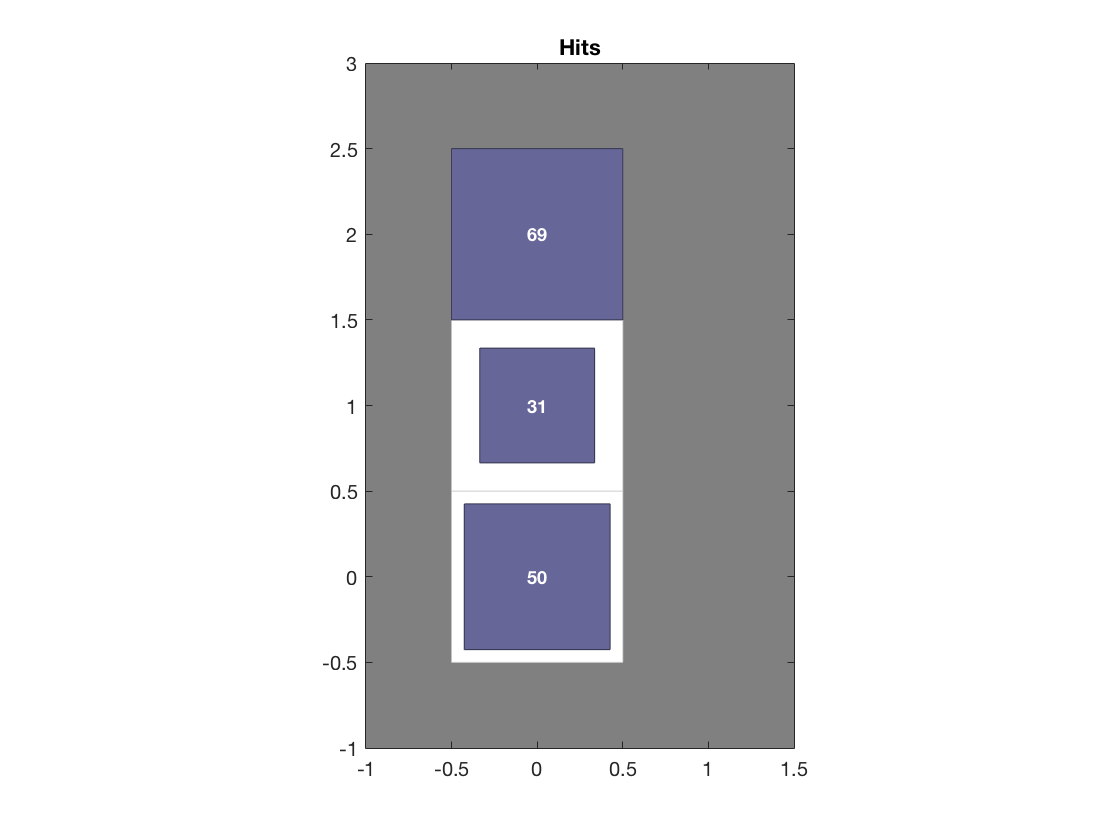
\includegraphics[width=0.49\linewidth]{img/somirisgrid}
    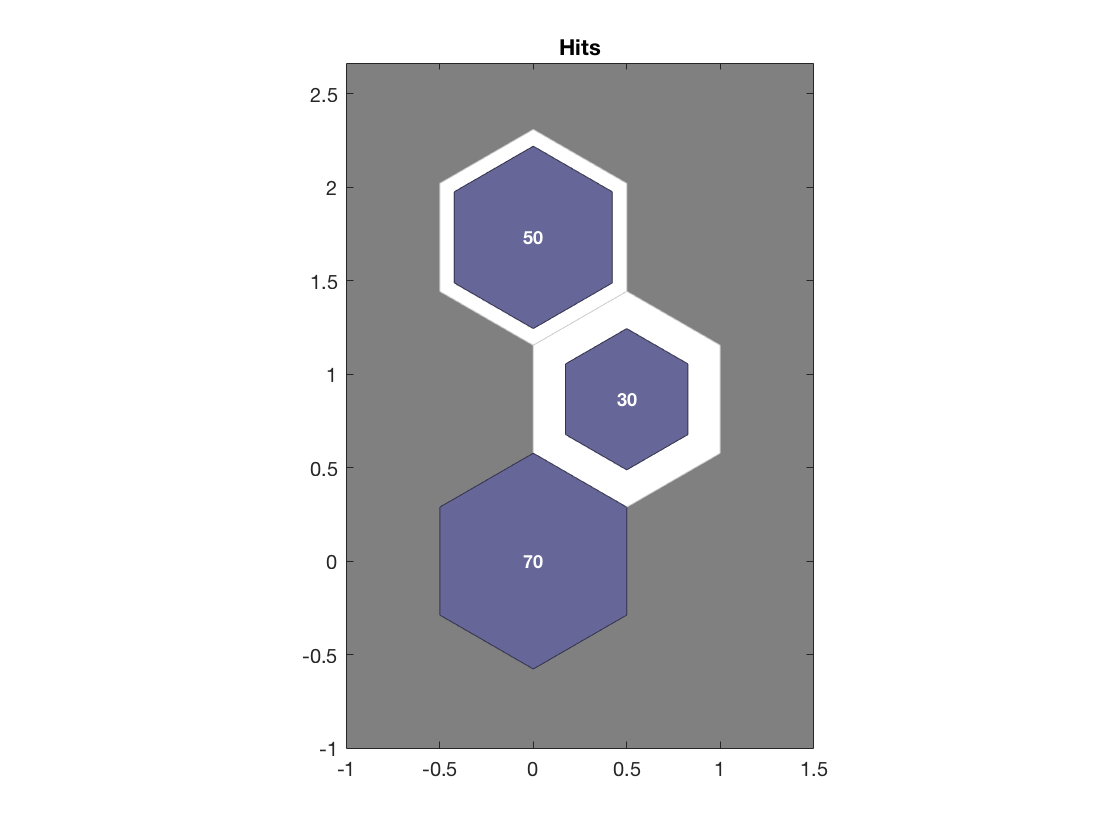
\includegraphics[width=0.49\linewidth]{img/somirishex}
  \end{center}

  If we look at the Adjusted Rand Index, the following results are obtained:
  \texttt{gridtop = 0.6719, hextop = 0.6719, randtop = 0.6828}. It is important
  to say that using \texttt{randtop} the ARI varies each time we train the network,
  as the shape of the clusters is stochastic.

  If the size of the grid is changed, the ARI decreases as expected.
 
\end{multicols}
\end{document}
